\documentclass[12pt,letterpaper,twoside]{article}
\usepackage{amsmath}
\usepackage{amsfonts}
\usepackage{appendix}
\usepackage[figurewithin=section,tablewithin=section]{caption}
\usepackage[usenames,dvipsnames]{color}
\usepackage{graphicx}
\usepackage{longtable}
\usepackage{rotating}
%\usepackage{verbatim}
\usepackage[pdftex,bookmarksopen=false]{hyperref}
%\usepackage[pdftex]{hyperref}
\hypersetup{pdfauthor={John Sibert}}
\hypersetup{pdfsubject={Assessment Model of MHI YFT Stocks}}
\hypersetup{pdftitle={Assessment model of Main Hawaiian Islands
Yellowfin Tuna Population}}
\hypersetup{pdfkeywords={yellowfin,state space, biomass transfer, model,Hawaii}}

\newcommand\doublespacing{\baselineskip=1.6\normalbaselineskip}
\newcommand\singlespacing{\baselineskip=1.0\normalbaselineskip}
\renewcommand\deg[1]{$^\circ$#1}
\newcommand\SD{SEAPODYM}
\newcommand\MFCL{MULTIFAN-CL}
\newcommand\ADMB{ADModel Builder}
\newcommand\SPC{Secretariat of the Pacific Community}
\newcommand\WCPO{Western Central Pacific Ocean}
\newcommand\SSAP{Skipjack Survey and Assessment Programme}
\newcommand\RTTP{Regional Tuna Tagging Programme}
\newcommand\PTTP{Pacific Tuna Tagging Programme}
\newcommand\FAD{fish aggregating device}
\newcommand\ADRM{advection-diffusion-reaction model}
\newcommand\help[1]{\color{Magenta}{\it #1 }\normalcolor}
\newcommand\widebar[1]{\overline{#1}}
\newcommand\EEZ{Exclusive Economic Zone}

\newcommand\None{{N_{1,1}}}
\newcommand\Ntwo{{N_{2,1}}}
\newcommand\Nsum{{N_{1,1}+N_{2,1}}}
\newcommand\peryr{yr$^{-1}$}
\newcommand\prevN[1]{{#1_{t-\Delta t}}}
\newcommand\nextN[1]{{#1_t}}


\title{Feasibility of developing stock assessment models for the
Main Hawaiian Islands Yellowfin Tuna Fishery}

\author{
John Sibert\thanks{sibert@hawaii.edu}\\
Joint Institute of Marine and Atmospheric Research\\
University of Hawai'i at Manoa\\
Honolulu, HI  96822 U.S.A.\\[0.125in]
\date{\today}
}

\pagestyle{myheadings}
\markboth{John Sibert\hfil MHI Yellowfin Assessment Model Feasibility}
{MHI Yellowfin Assessment Model Feasibility\hfil John Sibert}

\begin{document}
% amsmath package
\numberwithin{equation}{section}
\numberwithin{figure}{section}
\maketitle

%\doublespacing

\begin{abstract}
The yellowfin tuna fishery in the Main Hawaiian Islands (MHI)
is an important commercial and recreational fishery and
has a documented 65 year history. Local management of this fishery is
hampered by lack of stock assessment results specific to the MHI. The
feasibility of developing state-space Schafer model with ties to the
larger Pacific yellowfin population,
external forcing, Bayesian constraints, and robust estimation
specifically for the MHI was investigated. The models are feasible, but
parameter estimation is hindered by possible lack of an exploitation
signal in the data.
\end{abstract}

\section{Introduction}
The Main Hawaiian Islands (MHI) yellowfin tuna,
{\it Thunnus albacares}, (YFT) fishery is 
a small, but very important important fishery within the State of
Hawaii, and sustainable management of this
fishery is a local issue that deserves scientific support.
The documented history of the YFT fishery begins in
1949, predating statehood by 10 years, and is possibly a longer catch
history than that of the Japanese distant water longline fishery.
The MHI YFT population is, of course,
embedded in the much larger pan-Pacific stock, which also has a long
exploitation history and is the subject of on-going stock assessment
efforts by the Western and Central Pacific Fisheries Commission (WCPFC).
Many local fishermen in Hawaii
believe that the MHI supports a ``resident'' yellowfin population
which spawns and resides in the MHI.
Some scientific observations are consistent with this belief. 
Recent tagging and tracking
studies show that the rate of exchange between the MHI population
and the larger stock is low (Itano and Holland 2000). 
Analysis of YFT otoliths sampled from
throughout the Pacific conclude that 90\% or more of the MHI
population was spawned and reared in the MHI (Wells et al 2012).

Contemporary fisheries management often depends on results of stock
assessment models to establish quantitative fishery reference points
such as ``acceptable biological catch''.
Such models do not exist for the MHI YFT population, and
it is not clear that creating stock assessment model
for a single component of a shared stock is feasible.
The purpose of the work described in this report is to asses the
feasibility of developing stock assessment models for the MHI YFT
that link the MHI population to the larger Pacific population.


\section{Data}
\begin{figure}
\begin{center}
%\includegraphics[height=0.5\textheight]{./graphics/5_gear_catch_history_a.pdf}
\includegraphics[width=1.0\textwidth]{./graphics/5_gear_catch_history_a.pdf}
\caption{\label{fig:annualTS}
Annual yellowfin catch in metric tonnes by fisheries
operating in the Main Hawaiian Islands from combined HDAR and NOAA data.
}
\end{center}
\end{figure}

Two basic sources of catch data were used in this analysis:
quarterly time series of YFT catch weights reported to (1)
Hawaii Department of Aquatic Resources (HDAR) for several fishing
gears from 1949 to 2014 and (2)
to the National Oceanic and Atmospheric Administration (NOAA), National
Marine Fisheries Service for the Hawaii-based longline fleet
from 1995 through 2013 under the federally mandated log book program.  
The quarterly data from HDAR show clear seasonal variation and include
occasional zero observations between quarters with substantial
reported catch (Figure~\ref{fig:hdarTS}).
Whether these seasonal fluctuations and zero
catch observations represent changes in abundance, changes in
catchability, or changes in
fishery participation is unknown. In preliminary tests, the model appeared to
interpret catch variability as variability in stock abundance
predicting large fluctuations in biomass around the isolated zero
observations. Therefore, the quarterly data were aggregated by year
and used for all further model runs; see Figure~\ref{fig:annualTS}.
Statistical properties of the catch data and the method of joining the
HDAR and NOAA longline time series are elaborated in
Appendix~\ref{sec:data}. 


\begin{figure}[t]
\begin{center}
\includegraphics[width=1.0\textwidth]{./graphics/annual_region_2_biomass.pdf}
\caption{\label{fig:r2biomass}
Annual estimated biomass trends in MFCL Region 2 from the 2014 WCPFC YFT
stock assessment, Davies et al. 2014.
}
\end{center}
\end{figure}
A biomass exchange model presupposes a source source of biomass.
Model estimates of yellowfin biomass by \MFCL\ (MFCL)
from the most recent WCPFC stock assessment (Davies et al 2014) 
provide convenient estimates of immigrant biomass. 
The MHI straddle the boundary between MFCL regions 2 and 4.
Region 2 is arguably
more similar ecologically to the MHI than the more equatorial region
4, and the population in region 4 is much larger and exhibits a greater level
of depletion than the population in region 2, Figure~\ref{fig:MFCLregionB}.
The quarterly estimates for
region 2 were aggregated by year and used as the immigrant source for
model testing, Figure~\ref{fig:r2biomass}.
Since the MFCL assessment uses data for the period 1952 through 2012,
catch data outside of this period were excluded from this analysis.

\help{More background and discussion of data deficiencies is needed
here, e. g.  the ``ahi'' problem, HDAR reporting requirements, changes
in the database, and ``recreational'' data.}

Further properties of the data are presented in Appendix~\ref{sec:data}. 

\section{Models}
Two similar state-space models, both derived from a basic
Schaefer biomass dynamics model (Schaefer, 1954), were tested.
State-space models separate variability in the biological
processes in the system (transition model)
from errors in observing features of interest
in the system (observation model). 
The general form of the transition equation is
\begin{equation}
\alpha_t=T(\alpha_{t-1}) + \eta_t
\end{equation}
where the function $T$ embodies the stock dynamics mediating the
development of the state at time $t$ from the state at the previous
time with random process error, $\eta$.
The general form of the observation equation is
\begin{equation}
x_t = O(\alpha_t) + \varepsilon_t
\end{equation}
where the function $O$ describes the measurement process with
error $\varepsilon$ in observing the population.
Age-aggregated models were developed in preference to a more complex
age-structured model for examining the feasibility of a MHI YFT
assessment model.

Fishing mortality in both models is treated explicitly as a random walk
without recourse to effort standardization,
estimation of catchability coefficients, or creation of an
index of abundance based on catch per unit of effort (CPUE). 
The logarithm of fishing
mortality is assumed to
follow a random walk with normal increments, i.e.,
\begin{equation}
\log F_{g,t} = \log F_{g,t-1} + \xi_t;\quad \xi_t\sim
N(0,\sigma^2_F) \label{eqn:Fwalk}
\end{equation}
where  $\sigma^2_F$ is the variance of the fishing
mortality random walk.


\subsection{Two populations with explicit exchange}
The principle model assumptions are:
\begin{enumerate}
\item The Pacific Ocean is divided into two regions:
MHI (region 1) and elsewhere (region 2).
\item Fish immigrate from region 2 to region 1, and mix completely.
Immigrant fish are indistinguishable from ``local'' fish,
and the two components interact identically with the fishing gear in
region.
\item Fish emigrate from region 1 to region 2, but emigrant fish have
no effect on region 2 population dynamics, i.e., region 2 is an infinite
sink. Emigration is considered to be a source of mortality analogous
to ``natural'' mortality.
\item Immigration into the MHI is dependent on the
biomass of the yellowfin population outside of the MHI as estimated by
some other model, e.g., \MFCL\ (MFCL) or \SD. In the present model,
MFCL region 2 is assumed to be the source of immigrants (see previous
paragraph).
\item The fishery comprises several gear types or fleets, each
characterized by a distinct fishing mortality time series.
Fishing practices have evolved continuously over the 66 year history
of the fishery making estimation of satisfactory measures of fishing
effort difficult and contentious..
The evolution of fishing mortality for each fleet over time is
represented by a random walk,
i.e., the fishing mortality in the current time step is equal
to the fishing mortality in the previous time step plus a random
deviation.
\item Ninety percent of the fish resident in region 1 are assumed to
be locally spawned and reared (Wells et al 2012). 
This assumptions requires that the model to be able to track
the size of both the local and the immigrant subpopulations separately so
that the proportion local can be computed. It is
further assumed that this ratio has been nearly invariant since 1952.
\end{enumerate}

Full derivations of and all model equations arising from these
assumptions are presented in Appendix~\ref{sec:models}. The resulting
model is something like a state-space Schafer model with emigration,
external forcing, Bayesian constraints, and robust estimation.
Let $\None$ equal the biomass of fish originating in region~1
and residing in region~1
and $\Ntwo$ equal the biomass of fish originating in region~2
but residing in region~1.
The following pair of simultaneous non-linear differential equations
describe the dynamics of the two subpopulations.
\begin{eqnarray}
\label{eqn:coupledschaeferq}
\frac{d\None}{dt}&=&\None\Big[r\Big(1-\frac{\None}{K}\Big)
-F - T_{12}\Big] - (1-q)2r\frac{\None\Ntwo}{K}\nonumber\\
\\
\frac{d\Ntwo}{dt}&=&\Ntwo\Big[r\Big(1-\frac{\Ntwo}{K}\Big)
-F - T_{12}\Big] - q2r\frac{\None\Ntwo}{K} + T_{21}\nonumber
\end{eqnarray}
where $r$ is the logistic growth rate per year,
$K$ is the asymptotic biomass,
$F$ is the total fishing mortality in region~1, $T_{12}$
is the emigration rate from region~1 to region~2, and $T_{21}$
is the rate of immigration of biomass from region~2 to region~1.
The nonlinear mortality term $2r\frac{\None\Ntwo}{K}$ is a
consequence of assuming
two subpopulations constrained by the same logistic process.
The parameter, $q$, apportions the effects of the nonlinear
mortality term between the two subpopulation.

\subsection{Single population with indexed abundance}
The principle model assumptions are:
\begin{enumerate}
\item The dynamics of the population of YFT in the MHI follows a
simple Schaefer model is MHI-specific growth parameters.
\item The local dynamics are ```forced'' by assuming that the local
abundance is approximately proportional to the abundance of the larger
Pacific population.
\item Fishing mortality is represented by a random walk (as in the
two-population model).
\end{enumerate}

Thus the local dynamics follow the classic Schaefer form:
\begin{equation}
\label{eqn:ischaefer}
\frac{dN}{dt} = rN(1-\frac{N}{K}) - FN
\end{equation}
where $N$ is the biomass of YFT in the MHI, 
$r$ is the logistic growth rate per year,
$K$ is the asymptotic biomass, and
$F$ is the total fishing mortality per year in the MHI.

\section{Results}
\subsection{Two populations with explicit exchange}
\help{Preliminary results of the two population model were presented
in a previous report. More work has been done on model interpretation
and these previous results need revision.}

\subsection{Single population with indexed abundance}

\section{Discussion}

%The age-aggregated approach using a logistic model with emigration and
%immigration shows sufficient promise to continue model development.
%The general behavior of the model system (Figure~\ref{fig:simNN} and
%~\ref{fig:NNts}) appropriately describes a small persistent population
%interacting with a much larger one.
%The efficacy of the random walk
%representation of fishing mortality is particularly encouraging, and
%avoids debates about changes in catchability associated with
%changes in fishing efficiency.
%The proportion of local fish in the system is sensitive to model
%parameters and can effectively be constrained to be near the empirically
%determined value of 0.9. Coupling immigration to the output of
%some other model is relatively trivial to implement and is
%sufficiently flexible to use output from alternative models.
%
%Unfortunately, population dynamics parameters, with the possible
%exception of $q$, do not appear to be estimatable. Lack of
%sensitivity could be due to several causes: the model is completely
%ill-posed, the code is incorrect, there is no signal in data, or some
%combination of these. Inspection of catch trends
%(Figure~\ref{fig:annualTS}) does not reveal any obvious signs of stock
%depletion and recovery. Estimation of population dynamics parameters
%in a lightly exploited stock is a well-known problem in stock
%assessment.
%
%Figure~\ref{fig:NNphase} suggests that the model equations
%(\ref{eqn:coupledschaeferq}) have non-trivial equilibria for certain
%parameter values.
%The relationships between of the parameters $q$, $T^*_{21}$,
%and $\bar{p}$ are not clear.
%Estimation of fisheries reference point would be simpler if
%an analytic expression for the equilibrium point were available.
%Finite difference approximations of logistic population models are
%notoriously unstable under certain circumstances. An analytical
%solution of equation~\ref{eqn:coupledschaeferq} would be of great
%help.

\vspace{4ex}
%\clearpage
\noindent {\bf Acknowledgements.}
This work was funded by the Western Pacific Regional Fisheries
Managment Council. I thank the Council for its generous support and
Council Staff Paul Dalzell and Eric Kingma for encouraging me to
actually take on this challenging project and for their on-going
collaboration.
Thanks to Mr. David Itano for sharing insights into the small-boat
fisheries in Hawaii.
Thanks to Mr. Reginald Kokubun of the Hawaii Division of Aquatic
Resources for supplying catch report data from the HDAR commercial
fisheries data base.
Thanks to Mr. Keith Bigelow and Ms. Karen Sender of NOAA Pacific
Island Fisheries Science Center for supplying logbook reporting data and
weight-frequency data from the PIFSC data base.
Thanks also to Dr. John Hampton of the Secretariat of the Pacific
Community, Oceanic Fisheries Programme, for making available
MULTICAN-CL output files from the latest Western and Central Pacific
Fisheries Commission yellowfin tuna stock assessment, and to Mr. Nick
Davies for sharing R scripts and advice to decode the MFCL output files.

\section*{References}
{\parindent=0cm \small
\everypar={\hangindent=2em \hangafter=1}\par
%\doublespacing
%Adam, M. S., J. Sibert, D. Itano and K. Holland. 2003. Dynamics of
%bigeye (Thunnus obesus) and yellowfin tuna (T. albacares) in Hawaii's
%pelagic fishery: analysis of tagging data with a bulk transfer model
%incorporating size specific attrition. Fishery Bulletin 101(2):
%215-228.

Davies, N., S. Harley, J. Hampton, S. McKechnie. 2014. Stock
assessment of yellowfin tuna in the western and central pacific ocean.
WCPFC-SC10-2014/SA-WP-04.

Fournier, D. A., H.J. Skaug, J. Ancheta, J.Sibert, J. Ianelli, 
A. Magnusson, M. N. Maunder, A. Nielsen. 2012. AD Model Builder:
using automatic differentiation for forstatistical inference of highly
parameterized complex nonlinear models. Opti-mization Methods and
Software 27, 233–249.

Itano, D., K. Holland. 2000.  Movement and vulnerability of bigeye
(Thunnus obesus) and yellowfin tuna (Thunnus albacares) in relation to
FADs and natural aggregation points.Aquat. Living Resour. 13: 213-223.

Kleiber, P., J. Hampton, N. Davies, S. Hoyle, D. Fournier. 2014.
MULTIFAN-CL User’s Guide

Nielsen, A., C. Berg. 2014. Estimation of time-varying selectivity
in stock assessments using state-space models. Fisheries Research
158:96-101.

Quinn, T, R. Deriso. 1999. Quantitative fish dynamics. Oxford
University Press, New York.

Schaefer, M. B. 1954. Some aspects of the dynamics of populations
important to the management of the commercial marine fisheries. IATTC
Bull. 1(2):27-56.

Skaug, H., Fournier, D., 2006. Automatic approximation of the marginal
likelihood in non-Gaussian hierarchical models. Computational
Statistics \& Data Analysis 51, 699–709.

Wells, D., J. Rooker, D. Itano. 2012.  Nursery origin of yellowfin
tuna in the Hawaiian Islands. Mar. Ecol. Prog. Ser. 461:187-196. 
\par}

\clearpage


\section*{Appendix}
\appendix

\section{Catch Time Series}
\label{sec:data}
%The Hawaii longline fishery has a long history and changed radically
%in the 1990s when new vessels entered the fleet and fishing gear was
%modernized.
%The HDAR longline data covers the period 1949 through 2001 and does
%not differentiate between ``deep'' and ``shallow'' sets.
%The NOAA longline data covers the period 1995 through 2013 and reports deep
%and shallow set set separately.
%Thus the period of most radical change is included in time series.

%[1] Aku boat          Bottom/inshore HL Longline          Other            
%[5] Troll             Tuna HL           Casting           Hybrid           
%[9] Shortline         Vertical line    

% statistics of catch time series first differences
%TS                 Mean     S. D.
%OffshoreHL  0.017659002 0.5994987
%Troll       0.018124404 0.7051216
%Longline    0.002425213 0.7782023
%InshoreHL  -0.002342312 0.6935796
%AkuBoat    -0.004970204 1.0908600



The HDAR data comprise catch reports for the following gear
categories:
``Aku boat'', ``Bottom/inshore HL'', ``Longline'',  ``Troll'', ``Tuna
HL'', ``Casting'', ``Hybrid'',  ``Shortline'', ``Other'', and
``Vertical line''.
For this analysis catches by ``Casting'', ``Hybrid'',
``Shortline'', ``Other'', and ``Vertical line'' are combined into a new
category, ``Misc''. The ``Misc''
catches are highest after year 2000,
but comprise a very small proportion of the catch.
The catch time series for the HDAR data are shown in
Figure~\ref{fig:hdarTS}. These time
series exhibit marked annual cycles suggesting a strong seasonal
signal in the catches by all gears.
Some series also contain sustained periods of zero catch which
document the development and subsequent shift away from a specific
gear type. It is assumed that these declines in catches represent a
``collapse'' of a fishery due more to social and economic factors than
to a decline of stock.
Some time series are punctuated by brief episodes (one or two quarters in
length) of zero catches. Again, it is assumed that these zero catches
are not caused by low stock levels.

The longline fishery has changed drastically over time. In the late
1940s, it was a relatively small fishery using traditional
tarred rope gear making relatively shallow sets.
Participation in this fishery generally declined from 1950 to
late 1980s. In the 1990s, the longline
fishery expanded rapidly with the introduction of US fishing boats
from the Atlantic ocean using modern monofilament longline gear
capable of making both deep and shallow sets.

Figure~\ref{fig:hdarTS} also displays the first order differences
between successive quarters. This statistic emphasizes the seasonal
periodicity of all fishing gear and helps to identify potential anomalies in
the data such as changes in reporting protocols. 

The partial autocorrelations within each time
series are shown in Figure~\ref{fig:catchPACF}. These correlations
confirm the quarterly periodicity  of the catch time series.
The catch time series for Inshore HL, Longline, Troll, and Tuna HL show
similar patters with
significant positive autocorrelations at lags of 1, 3 and 4 quarters.
The autocorrelation pattern appears to be somewhat different for the Aku
boat catch time series.

NOAA began to collect data from the longline fleet under a federally
mandated logbook program in 1990, and in 1995, began to distinguish
deep and shallow sets in the data. The HDAR data do not
distinguish between deep and shallow sets.
Figure~\ref{fig:hdarnoaaLLTS} shows the correspondence between the
HDAR and NOAA time series. The combined deep plus shallow catches from
NOAA align fairly well with the overlapping HDAR data. The simple
average of the HDAR data with the combined NOAA deep plus shallow data
appears to have roughly the same autocorrelation structure as the
constituent time series, Figure~\ref{fig:LLpartialacf}.
Data are also available from NOAA for the period 1990-1995, but
have not yet been included in this analysis.

Histograms of first differences of the logarithm of catch time series
are shown in Figure~\ref{fig:diff1histo}. These differences are
clearly not normally distributed, indicating that a robust catch
likelihood might be useful.

\begin{figure}
\begin{center}
%\includegraphics[height=0.8\textheight]{./graphics/hdar_catch_history.pdf}
\includegraphics[width=\textwidth]{./graphics/hdar_catch_history.pdf}
\caption{\label{fig:hdarTS}
Yellowfin catch in metric tonnes by principle fisheries operating in
the Main Hawaiian Islands from the HDAR data.
The dotted red line superimposed on each time series is the difference in
catch between successive quarters.
The red tick marks on the abscissa indicate quarters where reported
catches were zero.
}
\end{center}
\end{figure}

\begin{figure}
\begin{center}
%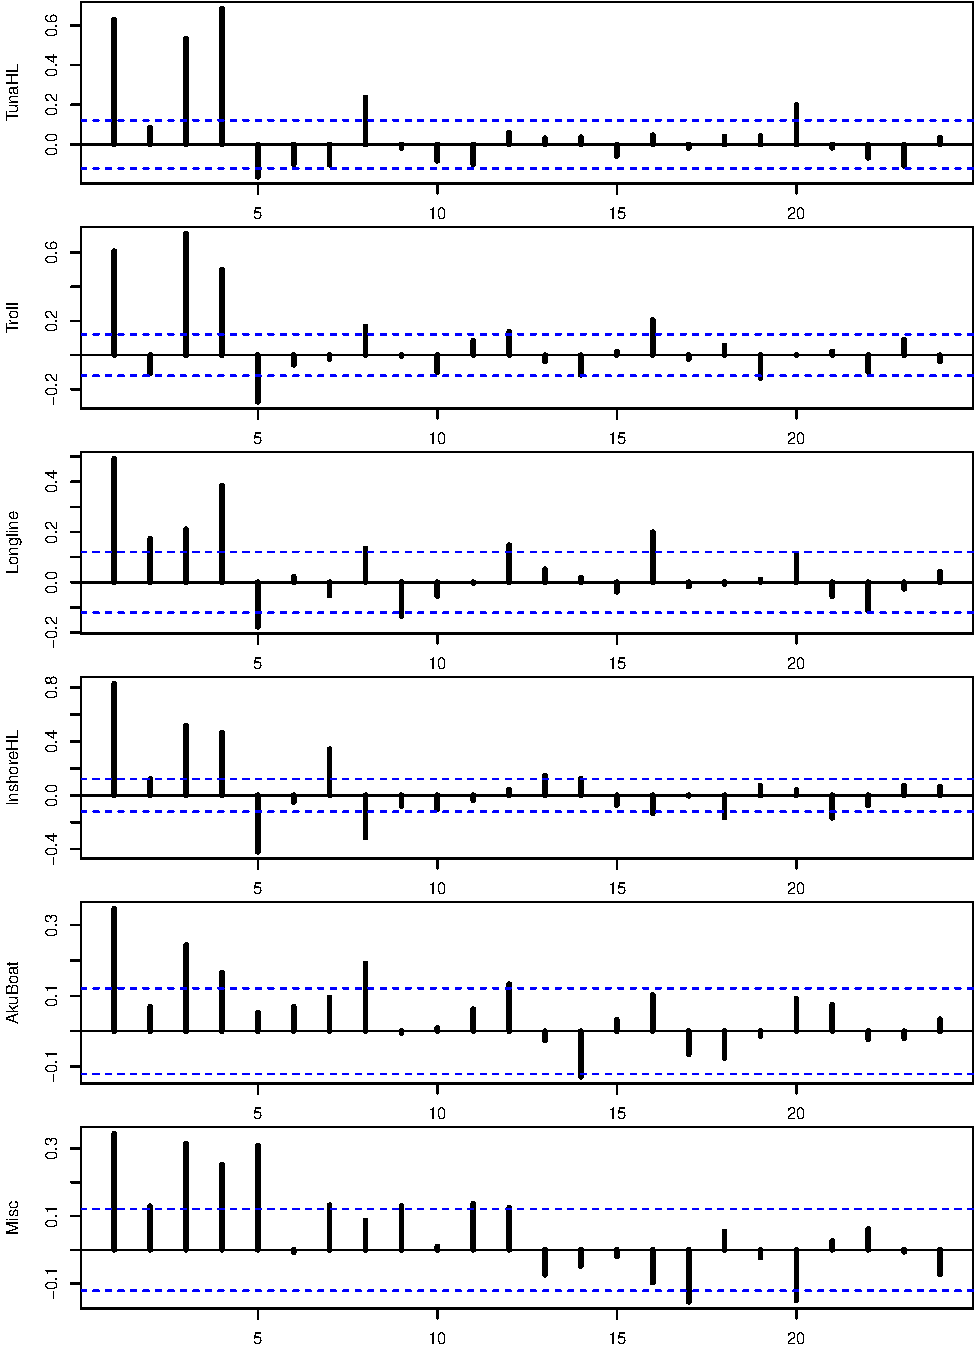
\includegraphics[height=0.8\textheight]{./graphics/partial_acf.pdf}
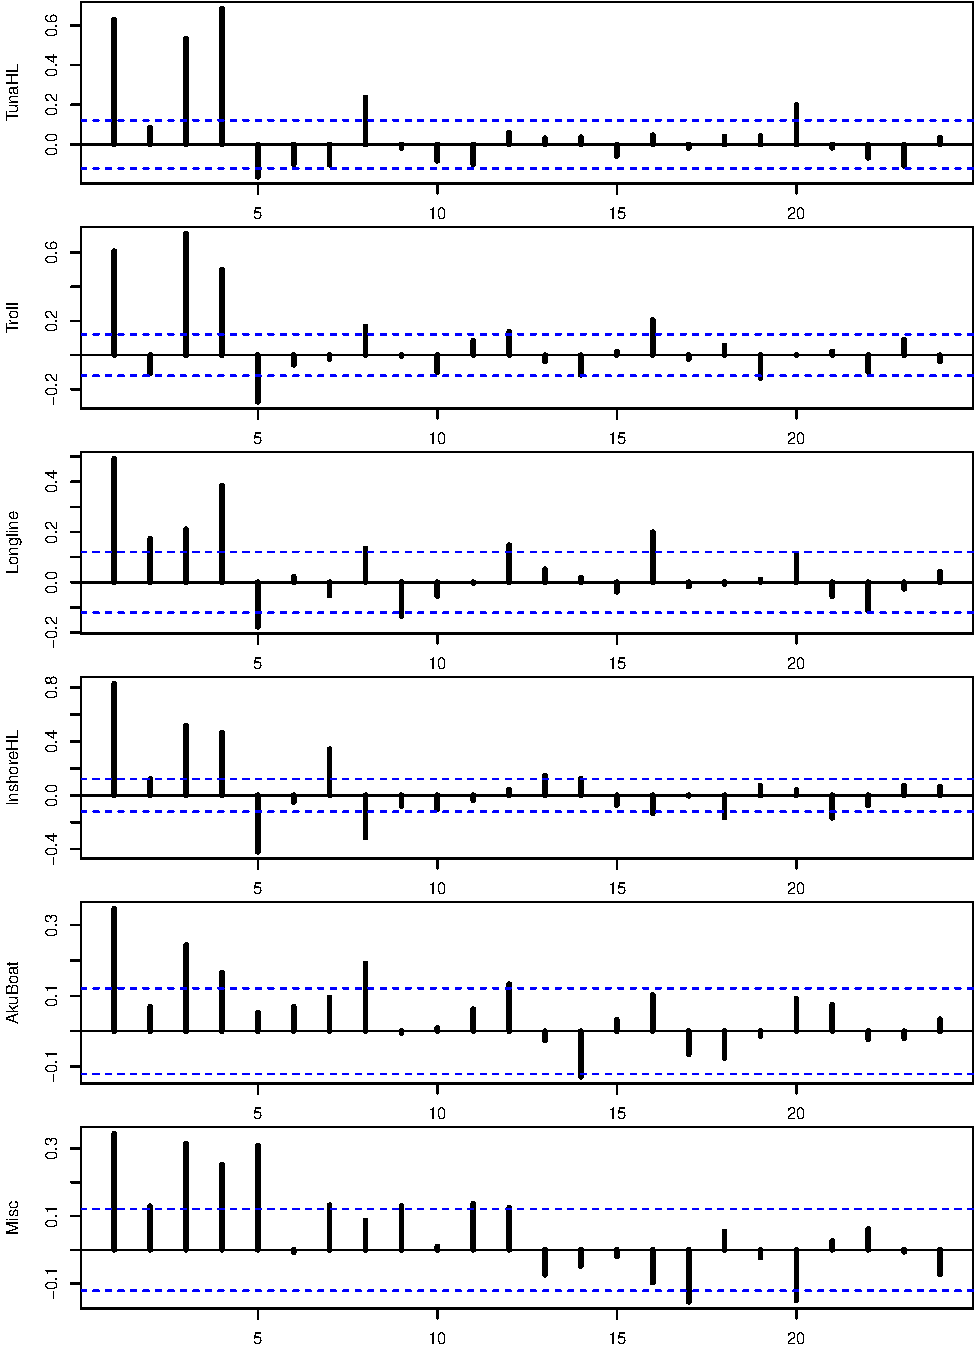
\includegraphics[width=0.8\textwidth]{./graphics/partial_acf.pdf}
\caption{\label{fig:catchPACF}
Partial autocorrelation coefficients of the HDAR catch time series. The
dashed blue lines indicate approximate 95\% confidence limits of the
correlations.}
\end{center}
\end{figure}

\begin{figure}
\begin{center}
%\includegraphics[height=0.8\textheight]{./graphics/hdar_noaa_LL_ts.pdf}
\includegraphics[width=\textwidth]{./graphics/hdar_noaa_LL_ts.pdf}
\caption{\label{fig:hdarnoaaLLTS}
Comparison between HDAR and NOAA longline time series. The upper panel
shows the NOAA deep and shallow set data superimposed on the HDAR
data. The lower panel shows the time series produced by a simple
average of the HDAR data and the sum of the NOAA deep and shallow
catches.}
\end{center}
\end{figure}

\begin{figure}
\begin{center}
%\includegraphics[height=0.8\textheight]{./graphics/LL_partial_acf.pdf}
\includegraphics[width=\textwidth]{./graphics/LL_partial_acf.pdf}
\caption{\label{fig:LLpartialacf}
Partial autocorrelations within the NOAA and combined time
series. F refers to the HDAR longline data, D refers to the NOAA deep
set data, S to the shallow set data,
DS to the combined deep and shallow set data, and Mean to the average
of the HDAR and NOAA deep plus shallow.
}
\end{center}
\end{figure}

\begin{figure}
\begin{center}
%\includegraphics[height=0.8\textheight]{./graphics/first_difference_histograms.pdf}
\includegraphics[width=\textwidth]{./graphics/first_difference_histograms.pdf}
\caption{\label{fig:diff1histo}
Histograms of first differences of the logarithm of catch time series. 
The blue line is
a normal distribution with the same mean and standard deviation as the
first differences. The red line is the equivalent standard Cauchy distribution.}
\end{center}
\end{figure}

\begin{figure}
\begin{center}
%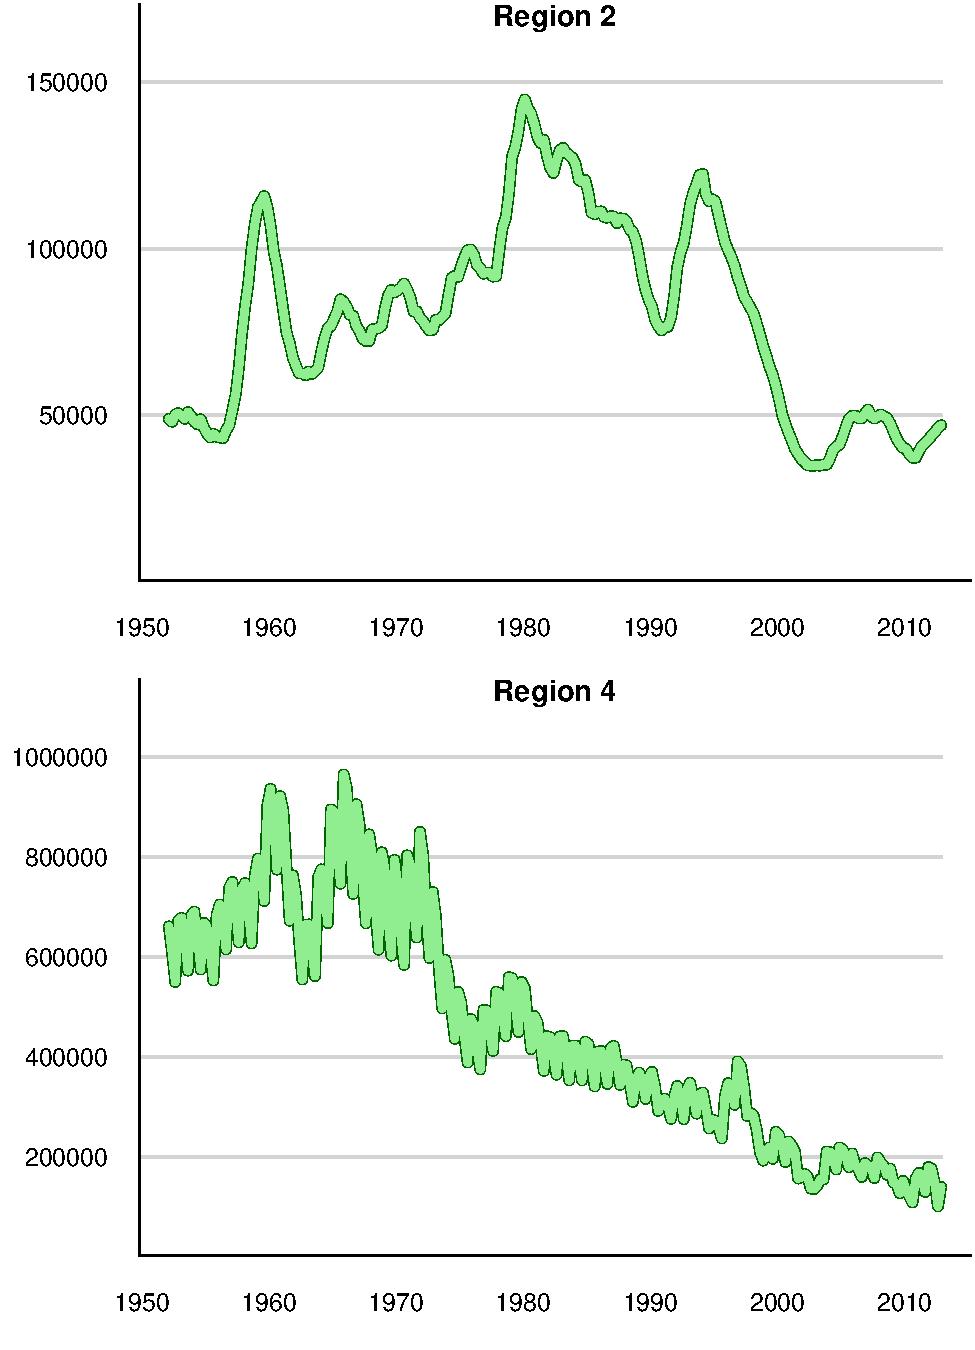
\includegraphics[height=0.8\textheight]{./graphics/MFCL_region_biomass.pdf}
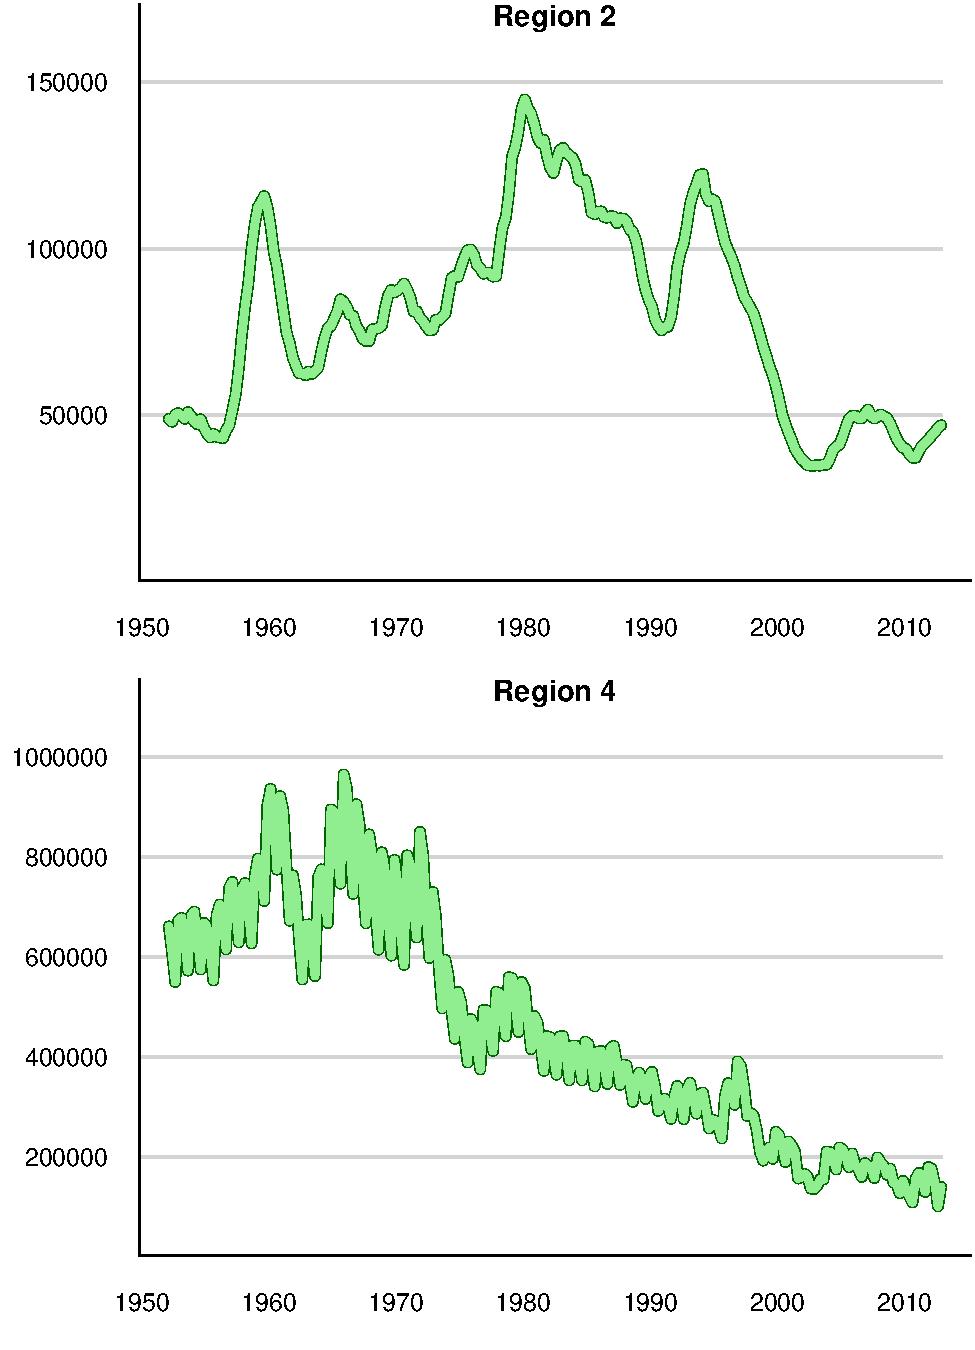
\includegraphics[width=\textwidth]{./graphics/MFCL_region_biomass.pdf}
\caption{\label{fig:MFCLregionB}
Quarterly biomass trends estimated in MFCL Regions 2 and 4 from the
2104 WCPFC YFT stock assessment, Davies et al. 2014.
}
\end{center}
\end{figure}


\clearpage
\section{Model development}
\label{sec:models}
\subsection{Two populations with explicit exchange}
%https://github.com/johnrsibert/XSSA/blob/master/ADMB/xssams.tpl
Let $\None$ equal the biomass of fish originating in region 1
and residing in region 1
and $\Ntwo$ equal the biomass of fish originating in region 2
but residing in region 1.
The total biomass of fish residing in region 1 is
$\Nsum$, and the dynamics of the population in region 1 is represented
as a modified Schaefer model:
\begin{equation}
\frac{d}{dt}\big(\Nsum\big)=\big(\Nsum\big)\Big[r\Big(1-\frac{\Nsum}{K}\Big)-F-T_{12}\Big]+T_{21}
\label{eqn:logistic}
\end{equation}
where $r$ is the logistic growth rate per year, $K$ is the
asymptotic biomass,
$F$ is the total fishing mortality in region 1, $T_{12}$
is the emigration rate from region 1 to region 2, and $T_{21}$
is the rate of immigration of biomass from region~2 to region~1.


An equivalent differential equation could be devised for the dynamics of
fish residing in region 2 
(i.e., $\frac{d}{dt}\big(N_{2,2}+N_{1,2}\big)$), but 
the dynamics of the fish population in region 2 is external to this
model. $T_{21}$ can be considered to be a form of population ``forcing''
by the larger stock in which the MHI population is embedded. $T_{21}$
could be a prediction from other models, such as \MFCL\ or \SD, 
in a sort of ``off-line'' coupling.

The appearance of
$\Nsum$ in the numerator of the logistic term reflects the assumption
that the population dynamics of immigrant fish depends on
the population dynamics in region 1. This assumption leads to an
important non-linearity in the model that predicts potential
overwhelming of one stock by the other.

The proportion of ``local'' fish $p = \frac{\None}{\Nsum}$ is an
important constraint, and it is necessary to model the two
subpopulations separately.
Equation~\ref{eqn:logistic} can be expanded and rearranged to become
\begin{eqnarray}
\label{eqn:coupledschaefer}
\frac{d}{dt}\big(\Nsum\big) &=&\None\Big[r\Big(1-\frac{\None}{K}\Big)
-F - T_{12}\Big] \nonumber\\
&+&\Ntwo\Big[r\Big(1-\frac{\Ntwo}{K}\Big)
-F - T_{12}\Big]  + T_{21}\\
&-& 2r\frac{\None\Ntwo}{K}\nonumber
\end{eqnarray}
The non-linear term, $2r\frac{\None\Ntwo}{K}$, in
equation~\ref{eqn:coupledschaefer} represents the reduction in biomass
of one population by the presence of the other population.
In order to represent
the two populations by separate equations, this
nonlinear term must be appropriately apportioned.
A new parameter, $q$, is introduced to accomplish the apportionment,
leading to a set of simultaneous non-linear differential equations for
the components of the population inhabiting region~1.
\begin{eqnarray}
\label{eqn:coupledschaeferqa}
\frac{d\None}{dt}&=&\None\Big[r\Big(1-\frac{\None}{K}\Big)
-F - T_{12}\Big] - (1-q)2r\frac{\None\Ntwo}{K}\nonumber\\
\\
\frac{d\Ntwo}{dt}&=&\Ntwo\Big[r\Big(1-\frac{\Ntwo}{K}\Big)
-F - T_{12}\Big] - q2r\frac{\None\Ntwo}{K} + T_{21}\nonumber
\end{eqnarray}

The log transformed equivalent of equation~\ref{eqn:coupledschaeferqa} is
\begin{eqnarray}
\label{eqn:coupledlogschaefer}
\frac{d\log(\None)}{dt}&=&r\Big(1-\frac{\None}{K}\Big) -F - T_{12} -
(1-q)2r\frac{\Ntwo}{K}\nonumber\\
\\
\frac{d\log(\Ntwo)}{dt}&=&r\Big(1-\frac{\Ntwo}{K}\Big) -F - T_{12} -
q2r\frac{\None}{K} + \frac{T_{21}}{\Ntwo}\nonumber
\end{eqnarray}

{\bf Transition Equation $T(\alpha_{t-1})$.}
The state space transition equation for the two components of the MHI
population is developed by solving
equations \ref{eqn:coupledlogschaefer} by finite differences
with explicit time stepping and adding process error
terms.
\begin{eqnarray}
\label{eqn:finitecoupledlogschaefer}
\log \None_t &=& \log \None_{t-\Delta t}\nonumber\\ 
             &+&\Delta t\bigg(r\Big(1-\frac{\None_{t-\Delta t}}{K}\Big)
-\sum_{g=1}^n F_{g,t-\Delta t} - T_{12} - (1-q)2r\frac{\Ntwo_{t-\Delta
t}}{K}\bigg)+\eta_t\nonumber\\
\\ \log \Ntwo_t &=& \log \Ntwo_{t-\Delta t}\nonumber\\
             &+&\Delta t\bigg(r\Big(1-\frac{\Ntwo_{t-\Delta t}}{K}\Big)
-\sum_{g=1}^n F_{g,t-\Delta t} - T_{12} - q2r\frac{\None_{t-\Delta t}}{K}
     +\frac{T_{{21}_{t-\Delta t}}}{\Ntwo_{t-\Delta t}}\bigg)+\eta_t\nonumber
\end{eqnarray}
where $\eta_t \sim N(0,\sigma_N)$
expresses process errors for both populations.

{\bf Behavior of model system.}
Efforts to derive an analytical expression to determine 
a meaningful equilibrium for equations~\ref{eqn:coupledlogschaefer}
have not been completely fruitful (Section \ref{sec:schaefer}).
Figure~\ref{fig:NNphase} shows phase plane diagrams for several
combinations of model parameters assuming constant $K$ and
$T_{21}$. Apparently the system tends towards
equilibrium with both $0 < \None \le K$ and $0 < \Ntwo \le K$ for some
combinations of model parameters.
The proportion of ``local'' fish, $p = \frac{\None}{\Nsum}$, depends on
the assumed value of $q$. For values of $q < 0.5$, the equilibrium
value of $p$ is less than 0.9. The functional relationship, if any,
between $p$ and $q$ is not clear, but it would appear that $q$ must be
be greater than $\simeq 0.5$ to achieve $p=0.9$.

The evolution of the model system in
equation~\ref{eqn:finitecoupledlogschaefer} with time is shown in
Figure~\ref{fig:NNts}. The system starts with $\None + \Ntwo = K$ and
$p=0.9$. After a few time steps the population decreases to reflect
influence of immigrants and the onset of fishing.
Towards the end of the simulation period the proportion local drops
below 0.9 in response to the decrease in the size of the immigrant
population.

\begin{figure}
\begin{center}
\includegraphics[width=1.00\textwidth]{./graphics/qcomp_4.pdf}
\caption{\label{fig:NNphase}
Phase plane for equation \ref{eqn:coupledlogschaefer}. Arrows represent
the trajectory of the system for different combinations of $\None$ and
$\Ntwo$; dashed red  line indicates $K = 1$; dashed green lines indicate
different values of $p$. The thick light green line indicates $p=0.9$.
Values of $q$ and $T_{21}$ are shown in each panel.
Other parameter values: $r=0.3, K=1.0, F = 0.007, T_{12}=0.01$.
}
\end{center}
\end{figure}

\begin{figure}
\begin{center}
\includegraphics[width=1.00\textwidth]{./graphics/sim_default_NNts.pdf}
\caption{\label{fig:NNts}
Behavior of equations \ref{eqn:finitecoupledlogschaefer} over time with
forcing from MFCL region 2 biomass (Figure~\ref{fig:MFCLregionB}) and
fishing mortality by fleet set proportional to observed catch.
Light blue lines indicate population components as indicated; 
dashed blue line indicates $K$;
solid red line indicates the proportion local, $p$;  
dashed red line line indicates $p=0.9$.
Other parameter values: $q=0.54, r=0.3, K=200000, T12=0.01, T21=0.002$.
}
\end{center}
\end{figure}

%Parameterization of $T_{21}$
{\bf Population Forcing.}
Immigration of stock from region 2 to region 1 is a
form of forcing whereby events outside of the model influence the
model dynamics. The term $T_{{21}_t}$ in 
equation~\ref{eqn:finitecoupledlogschaefer}
is the biomass immigrating
into the MHI stock at each time step. 
The likely candidates for forcing are MFCL regions 2 and 4, both of
which overlap the MHI. The estimated biomass trajectories for these
two regions are shown in Figure~\ref{fig:MFCLregionB}.
For testing purposes,
I assume that the source of immigrants is MFCL region 2, so that
\begin{equation}
T_{{21}_t} = T^*_{21}\cdot B_{2,t}
\end{equation}
where $B_{2,t}$ is biomass in region 2 at time $t$ taken from the MFCL output file
{\tt plot-12.par.rep} from the 2014 WCPFC stock assessment
(Davies et al 2014). $T^*_{21}$ is the proportion on
$B_{2,t}$ which migrates at each time step.

{\bf Asymptotic biomass.}
$K$ is the asymptotic biomass in a population growing according to
logistic dynamics. It is the population size to which the population
tends at equilibrium and is often dubbed ``carrying capacity''. 
It is not clear that a coupled logistic model such as equation~
\ref{eqn:logistic} has a non-trivial equilibrium. 
Given that the model forcing $B_{r,t}$ is not constant and that the
fishery is developing in a period of profound change in the oceans,
it is difficult to justify the assumption that the equilibrium
population size, $K$, has been constant for over 65 years. An
alternative parameterization for $K$ is to assume a random walk, for
example,
\begin{equation}
\log K_t = \log K_{t-1} + \omega_t;\quad \omega_t\sim
N(0,\sigma^2_\omega) \label{eqn:Kwalk}
\end{equation}
where  $\sigma^2_\omega$ is the variance of the
asymptotic population size random walk.
This parameterization was implemented in computer code, but not extensively
tested.

{\bf Observation Equation, $O(\alpha)$.}
Predicted catch in region 1 is the product of fishing mortality
and the total population in region, $\None+\Ntwo$.
Thus the state-space observation model predicting catch in the region 1
under this model is
\begin{equation}
\log C_{g,t} = \log \Biggl(F_{g,t}\cdot\Bigl(\frac{\None_{t-\Delta t}+\None_t}{2}
                           +\frac{\Ntwo_{t-\Delta
t}+\Ntwo_t}{2}\Bigr)\Biggr) + \varepsilon_t
\label{eqn:obs2}
\end{equation}
where the total population in region 1 is the sum of the average
population over the time step (Quinn and Deriso, 1999), and
$\varepsilon_t$ is a robust likelihood given by
\begin{equation}
\varepsilon_t \sim (1-a_g)*N(0,\sigma^2_\varepsilon)+a_g*C(0,\sigma^2_\varepsilon).
\end{equation}
C is the standard Cauchy probability density and $a_g$ is a
fleet-specifc proportion of ``contamination'' by the fat-tailed Cauchy
distribution. In practice $a_g = 0.07\; g=1\ldots n$.

{\bf Constraint on ``Proportion Local''.}
Proportion local is defined as $p = \frac{\None}{\Nsum}$. The logit
transformed proportion local, $L(p)$, is assumed to be normally
distributed around a mean value, $L(\bar{p})$.
\begin{equation}
\label{eqn:LpropL}
L(p)\sim N(L(\bar{p}),\sigma^2_{L(p)}).
\end{equation} 
$p$ is generally assumed to be approximately $0.9$. By varying the
value of the variance, $\sigma^2_{L(p)}$, $p$ can be made as
close to $0.9$ as is prudent.
This representation of $p$ can be interpreted as a Bayesian prior.
In principle, it may be possible to
estimate $\bar{p}$ and $\sigma^2_{L(p)}$, but interactions with
the parameter $q$ in equation~\ref{eqn:coupledschaeferq} should be
explored.

{\bf Estimation.} The model states, $\alpha_t$, are assumed to be random
effects (Skaug and Fournier 2006). Model parameters are estimated by
maximizing the joint likelihood of the random
effects and the observations.
\begin{equation}
L(\theta,\alpha,x)=
\prod^m_{t=2}\big[\phi\big(\alpha_t-T(\alpha_{t-1}), \Sigma_\eta\big)\big]
\prod^m_{t=1}\big[\phi\big(x_t-O(\alpha_t), \Sigma_\varepsilon\big)\big]
\end{equation}
Here, $m$ is the number of time steps in the catch time series and
$\theta$ is a vector of model parameters. A complete list of
parameters is found in Table~\ref{tab:allvars2}. 
The model is implemented in ADMB-RE (Fournier et al 2012).
The actual number of
parameters to be estimated depends on the model configuration,
specified by phase flags in the input file. 
%All computer code, data files, and draft reports in support of this
%analysis can be found at Github:\linebreak
%\url{https://github.com/johnrsibert/XSSA.git}.


\begin{table}
\caption{Complete list of variables and parameters for the two
population model
\label{tab:allvars2}}
\begin{center}
\begin{tabular}{ll}
\hline
Variable & Definition\\
\hline
\hline
$m$ & Number of quarterly time steps\\
$n$ & Number of fishing gears\\
\hline
\hline
$r$ & Instantaneous growth rate $(y^{-1})$\\
$K$ & Asymptotic biomass (mt) \\
$T_{12}$ & Emigration rate $(y^{-1})$\\
$T^*_{21}$& Immigration rate $(y^{-1})$\\
$q$ & Nonlinear mortality apportionment proportion\\
\hline
$\sigma_N$ & Population growth SD\\
$\sigma_F$ & Fishing mortality random walk SD\\
$\sigma_Y$ & Observation error SD \\
$a$ & Likelihood contribution from fat-tailed distribution\\
\hline
$\bar{p}$ & Mean proportion local\\
$\sigma_{L(p)}$ & SD logit transformed $\bar{p}$\\
\hline
\end{tabular}
\end{center}
\end{table}

\clearpage
\subsection{Single population with indexed abundance}
The indexed abundance model\footnote{https://github.com/johnrsibert/XSSA/blob/master/ADMB/issams.tpl}
assumes that the biomass of YFT in the MHI
is proportional to the biomass of an ``index'' population.
Let $I_t$ equal the biomass of the index population and $Q$ the
constant of proportionality between the MHI population and the index
population, thus
\begin{equation}
\label{eqn:Qprop}
\varphi_t \sim N(QI_t-N_t,\sigma_Q)
\end{equation}
becomes a component of the total likelihood due to differences between
the MHI biomass and the index population biomass.


{\bf Transition Equation $T(\alpha_{t-1})$.}
The state space transition equation for the single population model is
developed by solving \ref{eqn:ischaefer} analytically from one time to
the next (see Section \ref{sec:schaefer}).
\begin{equation}
%\label{eqn:intschaefer}
N_t = \frac{K(r-\bar{F}_t)}{\frac{K(r-\bar{F}_t)}{N_{t-\Delta t}}e^{-\Delta
t(r-\bar{F}_t)}-re^{-\Delta t(r-\bar{F}_t)} -r} + \eta_t
\end{equation}
where 
$\bar{F}_t$ is the total fishing mortality, i. e.,
$$
\bar{F}_t =\sum_{g=1}^n F_{g,t-\Delta t}.
$$
$\eta_t \sim N(0,\sigma_N)$ is the process error expressing
variability in population dynamics.


{\bf Observation Equation, $O(\alpha)$.}
Predicted catch, $\widehat{C}_{g,t}$, for each gear is the product of
estimated fishing mortality and the total biomass.
\begin{equation}
\log \widehat{C}_{g,t} = \log\bigg(F_{g,t}\cdot\Bigl(\frac{N_{t-\Delta
t}+N_t}{2}\Bigr)\bigg) + \varepsilon_t
\label{eqn:obs1}
\end{equation}
where the total biomass is  the average
biomass over the time step (Quinn and Deriso, 1999), and
$\varepsilon_t$ is a ``zero-inflated'' normal likelihood given by
\begin{equation}
  \log \varepsilon_t = \left\{
    \begin{array}{r@{\;:\quad}l}
       C_{g,t} > 0 &
(1-p_0)\cdot\bigg(\log\frac{1}{\sqrt{2\pi\sigma^2_Y}}
          -\Bigl(\frac{\log
C_{g,t}-\log\widehat{C}_{g,t}}{\sigma_Y}\Bigr)^2\bigg)\\
       C_{g,t} = 0 & p_0 \cdot\log \frac{1}{\sqrt{2\pi\sigma^2_Y}}\\
    \end{array}
  \right.
\end{equation}
$p_0$ is the proportion of observed catch observations equal to 0.0.
This proportion may be estimated or fixed at a constant value. For
current analysis, it is fixed at $p_0 = 0.15738$ as computed from the data.
% line 186, file issams.cpp, prop_zero =  0.4918 0 0 0.098361 0.19672, tprop_zero = 0.15738



\begin{table}
\caption{Complete list of variables and parameters for the single
population model.
\label{tab:allvars1}}
\begin{center}
\begin{tabular}{ll}
\hline
Variable & Definition\\
\hline
\hline
$m$ & Number of quarterly time steps\\
$n$ & Number of fishing gears\\
\hline
\hline
$r$ & Instantaneous growth rate $(y^{-1})$\\
$K$ & Asymptotic biomass (mt) \\
$Q$ & Abundance index proportionality constant\\
$p_0$ & Proportion of zero catch observations;\\
      & fixed at $p_0 = 0.15738$\\
\hline
$\sigma_N$ & Population growth SD\\
$\sigma_F$ & Fishing mortality random walk SD\\
$\sigma_Q$ & Abundance index proportionality SD\\
$\sigma_Y$ & Observation error SD \\
\hline
\end{tabular}
\end{center}
\end{table}
\clearpage
\section{Integrating Schaefer Models}
\label{sec:schaefer}
The widely used Schaefer (1954) fisheries stock assessment model 
is a simple
extension of the logistic population model with a term added to
represent removals from the population due to fishing.
\begin{equation}
\label{eqn:sschaefer}
\frac{dN}{dt} = rN(1-\frac{N}{K}) - FN = N(r-F-\frac{r}{K}N)
\end{equation}
where $N$ is the population size,
$r$ is the instantaneous growth rate ($t^{-1}$),
$K$ is the asymptotic population size in the same units as $N$,
and $F$, is the instantaneous rate of removal due to fishing ($t^{-1}$).
Equation (\ref{eqn:sschaefer}) reduces to the logistic model
if $F$ is assumed to be zero.
These models are usually integrated numerically with
``explict'' finite difference methods to compute an approximation 
of the value of $N$ at some time. 
Such approximations are often unstable for 
values of $r$ large relative to the time step used in the finite
difference solution.
The performance of estimation methods in which logistic models
are embedded in a statistical procedure depending on numerical function
minimizers, i.e, models build using ADMB, TMB and BUGS,
is greatly improved in accuracy, speed and use of
computing resources if analytical solutions are used in preference
to finite difference approximations. 

\subsection{Single population}
Quinn and Deriso (1999) show the integral of the logistic ODE and
point out that it can be obtained using integration by partial fractions.
Numerous mathematics tutorials can be found on the World Wide Web use
integration of the logistic ODE to illustrate the technique of
integration by partial fractions.
The same procedure can be used to integrate the Schaefer ODE.
Equation~(\ref{eqn:sschaefer}) is rearranged slightly and variables
separated to become
\begin{equation}
\frac{K}{N(K(r-F)-rN)}dN=dt.
\end{equation}
The fraction in the left hand side can be factored into two parts,
\begin{equation}
\frac{K}{N(K(r-F)-rN)}=\frac{A}{N}+\frac{B}{(K(r-F)-rN)}.
\end{equation}
$A$ and $B$ are constants that can be found by solving
$K=A(K(r-f)-rn))+BN$
setting $N=K$ and $N=0$; 
$A=\frac{1}{r-F}$ and $B=1+\frac{F}{r-F}$.
The desired integral becomes
\[\int\frac{K}{N(K(r-F)-rN)}dN   = \int dt\]
\[\int\frac{A}{N}dN + \int\frac{B}{K(r-F)-rN}dN  = \int dt\]
\[\frac{1}{r-F}\int\frac{1}{N}dN + (1+\frac{F}{r-F})\int\frac{1}{K(r-F)-rN}dN  = \int dt\] 
\[\frac{1}{r-F}\log |N| + \frac{1}{r}(1+\frac{F}{r-F})\log |K(r-f)-rN| +log C  = t\] \[\log |N| - \log |K(r-F)-rN| + log C  = t(r-F)\]
\[\frac{|N|}{|K(r-F)-rN|}\cdot C  =  e^{t(r-F)}\]
\[\frac{|K(r-F)-rN|}{C|N|} =  e^{-t(r-F)}\]
where $C$ is the constant of integration.
Setting $|N| = N_t$, the population size at time $t$, yields
\begin{equation}
\label{eqn:NtC}
N_t=\frac{K(r-F)}{Ce^{-t(r-F)}+r}
\end{equation}
A formula suitable for computing population size at successive
time steps can be found by setting $N_t = N_{t-\Delta t}$ at time
$t=t-\Delta t$ in equation (\ref{eqn:NtC}).
The integration constant, $C$, becomes
\begin{equation}
C=\Bigg(\frac{K(r-f)}{N_{t-\Delta t}}-r\Bigg)e^{(t-\Delta t)(r-F)},
\end{equation}
and finally
\begin{equation}
\label{eqn:intschaefer}
N_t = \frac{K(r-F)}{\frac{K(r-F)}{N_{t-\Delta t}}e^{-\Delta t(r-F)}-re^{-\Delta t(r-F)} -r}
\end{equation}
\help{
Further simplification of this equation may be possible, but I have
not found it. In any case, equation (\ref{eqn:intschaefer}) is the
only general solution of the Schaefer ODE that I have seen, and it appears
to work well in numerical applications.
}

\subsection{Two populations with exchange}
The motivation for the two popultion Schaefer model with exchange is
developed fully in Appendix~\ref{sec:models}.

The basic equations can be written
\begin{eqnarray}
\label{eqn:xschaefer1}
\frac{d\None}{dt}&=&\None\Big(r-F-T_{12}-2(1-q)\frac{r}{K}\Ntwo-\frac{r}{K}\None\Big)\\
\nonumber\\
\label{eqn:xschaefer2}
\frac{d\Ntwo}{dt}&=&\Ntwo\Big(r-F-T_{12}-2q\frac{r}{K}\None-\frac{r}{K}\Ntwo\Big)+T_{21}
\end{eqnarray}
where $\None$ the biomass of fish originating in region~1
and residing in region~1,
and $\Ntwo$ is the biomass of fish originating in region~2
but residing in region~1.
The parameters $r$, $K$ and $F$ are unchanged from
equation~(\ref{eqn:sschaefer}), and
$T_{12}$ is the emigration rate from region~1 ($t^{-1}$), 
$T_{21}$ is the rate of immigration of biomass from region~2 to
region~1 in units of biomass per time,
and $q;\; (0 < q < 1)$ partitions the mortality caused by ``competition''
between the two subpopulations.
Substitute
\begin{eqnarray}
\label{eqn:Zdef}
Z_1&=&F+T_{12}+2(1-q)\frac{r}{K}\Ntwo\\
\nonumber\\
Z_2&=&F+T_{12}+2q\frac{r}{K}\None
\end{eqnarray}
into equations~(\ref{eqn:xschaefer1}) and~(\ref{eqn:xschaefer2})
respectively to produce model equations in a similar form to
equation~(\ref{eqn:sschaefer})
\begin{eqnarray}
\label{eqn:xschaeferZ1}
\frac{d\None}{dt}&=&\None(r-Z_1-\frac{r}{K}\None)\\
\nonumber\\
\label{eqn:xschaeferZ2}
\frac{d\Ntwo}{dt}&=&\Ntwo(r-Z_2-\frac{r}{K}\Ntwo)+T_{21}.
\end{eqnarray}
Equation~(\ref{eqn:xschaeferZ1}) can be integrated in the same manner as
equation~(\ref{eqn:sschaefer}) to yield
\begin{equation}
\label{eqn:N1tC}
\None_t=\frac{K(r-Z_1)}{C_1e^{-t(r-Z_1)}+r}.
\end{equation}

\help{All that remains is to find an equivalent integral for
equation~(\ref{eqn:xschaeferZ2}) and a means to simultaneously solve
for $C_1$ and $C_2$. }

%\begin{equation*}
%{{2\,\log \Big|{{2\,a\,x-\sqrt{b^2-4\,a\,c}+b}\over{2\,a\,x+
% \sqrt{b^2-4\,a\,c}+b}}\Big|}\over{\sqrt{b^2-4\,a\,c}}}+C=t
%\end{equation*}
%
%\begin{equation*}
%x=-{{\sqrt{b^2-4\,a\,c}\,\left(e^{{{\sqrt{b^2-4\,a\,c}\,t
% }\over{2}}-{{\sqrt{b^2-4\,a\,c}\,C}\over{2}}}+1\right)+b\,\left(e^{
% {{\sqrt{b^2-4\,a\,c}\,t}\over{2}}-{{\sqrt{b^2-4\,a\,c}\,C}\over{2}}}
% -1\right)}\over{a\,\left(2\,e^{{{\sqrt{b^2-4\,a\,c}\,t}\over{2}}-{{
% \sqrt{b^2-4\,a\,c}\,C}\over{2}}}-2\right)}}
%\end{equation*}
%
%
\clearpage
%\input{N1}
%\input{N2}


\end{document}
